%=====================================================================
\section{Negative winding: the bulk stays positive}\label{sec:mirror}
With winding $-|k|$ the wall must carry at least $2|k|$ $-\half$ defects. $-\half$ defects do not self-propel, so a positive bulk
cannot come from wall defects swimming off; and the excess over the natural $+1$ of a homeotropic disc is $-(|k|+1)$, not
$k-1$, so the two signs are not mirror images even topologically. Data: 570 active runs ($\rho\le0.15$, 3 seeds), same
grid and outputs as the positive sweep. Bulk charge = height of the positive peak of $Q(r)$ before the plunge to $-|k|$
(Sec.~\ref{sec:methods-knee}).
\begin{figure}[H]\centering
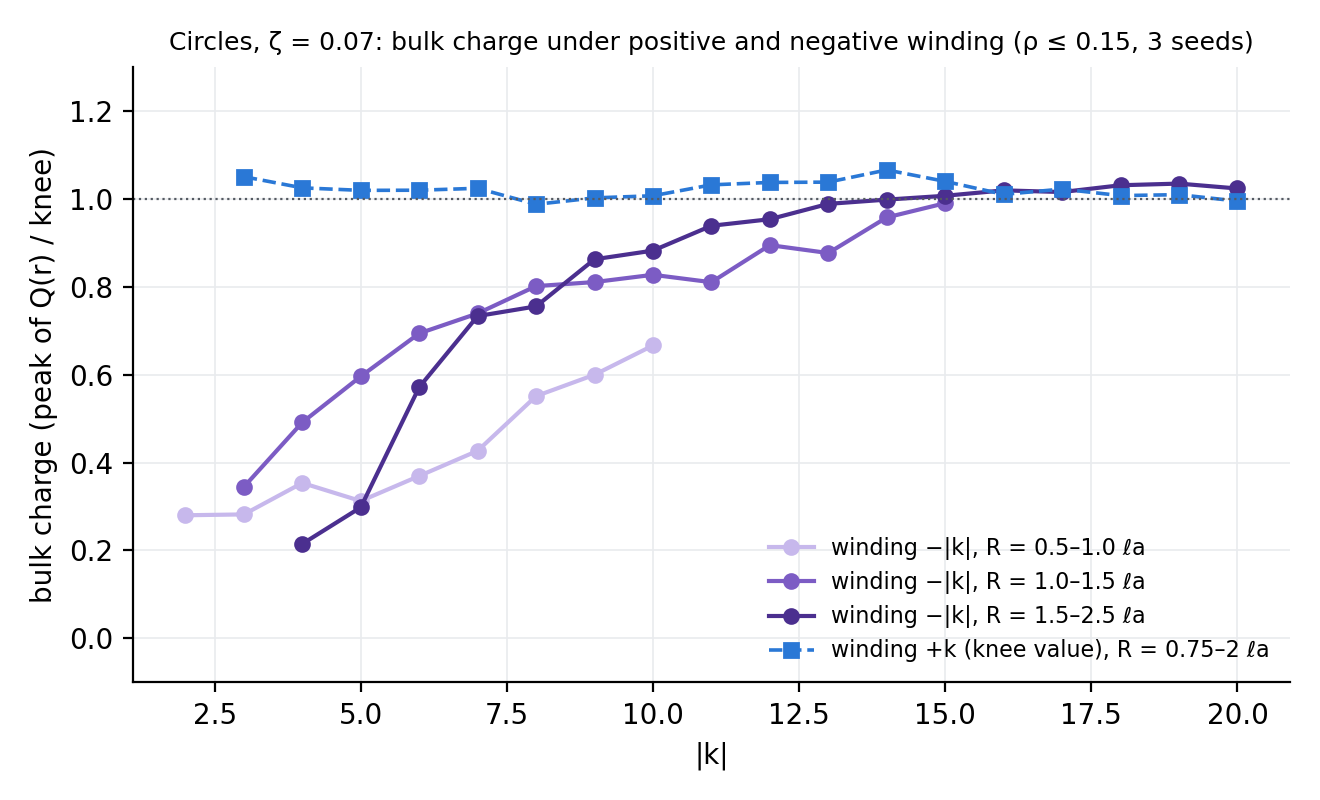
\includegraphics[width=0.78\textwidth]{mirror_bulk_vs_k.png}
\caption{Bulk charge against $|k|$: positive winding (knee value) and negative winding (peak of $Q(r)$), $\rho\le0.15$.}\label{fig:mirror}
\end{figure}
\begin{figure}[H]\centering
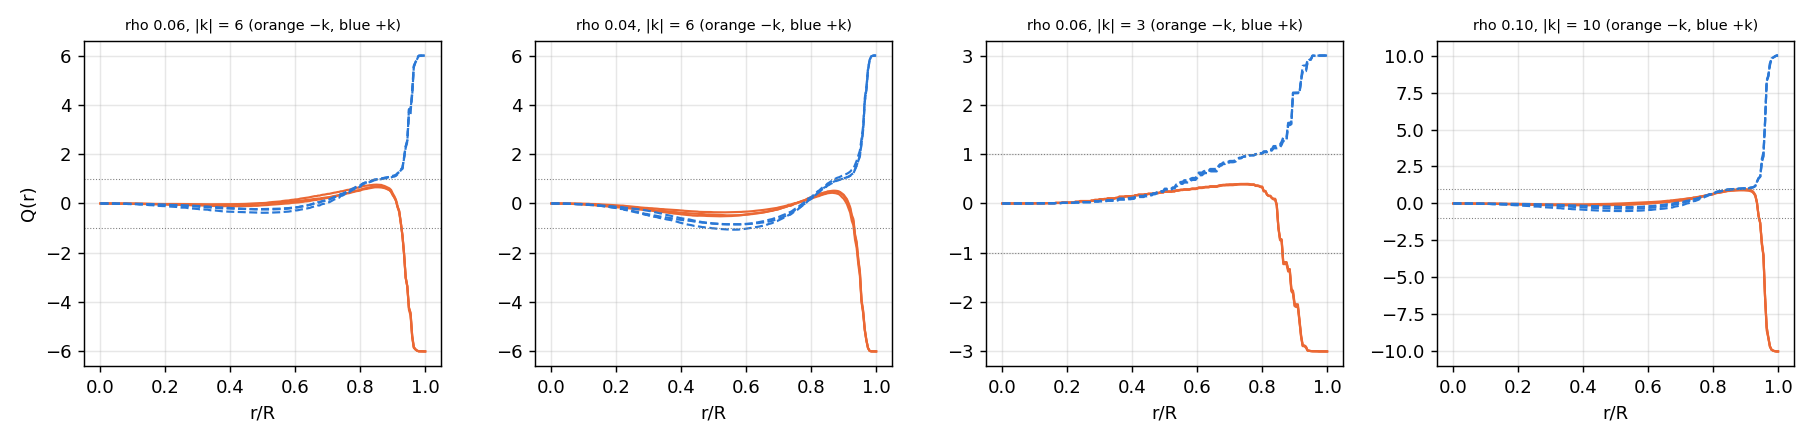
\includegraphics[width=0.85\textwidth]{mirror_Q_check.png}
\caption{Examples of $Q(r)$ with negative winding: a positive peak inside, then the plunge to $-|k|$ at the wall.}\label{fig:mirrorQ}
\end{figure}
\begin{table}[H]\centering\small
\caption{Mirror runs: mean peak $Q$ (bulk charge) over $\rho$ and seeds, and wall $-\half$ per frame; $2|k|$ = forced,
$2|k|+2$ = what a $+1$ bulk needs.}\label{tab:mirror}
\begin{adjustbox}{max width=\textwidth}
\begin{tabular}{rcccc|rcccc}\toprule
$|k|$ & bulk & range & wall $-\half$ & ($2|k|$, $2|k|+2$) & $|k|$ & bulk & range & wall $-\half$ & ($2|k|$, $2|k|+2$)\\\midrule
2 & 0.09 & 0.00--0.34 & 3.78 & (4, 6) & 12 & 0.92 & 0.82--1.02 & 25.20 & (24, 26)\\
4 & 0.27 & 0.00--0.52 & 7.83 & (8, 10) & 14 & 0.96 & 0.85--1.03 & 29.46 & (28, 30)\\
6 & 0.47 & 0.00--0.76 & 11.71 & (12, 14) & 15 & 1.00 & 0.94--1.08 & 31.74 & (30, 32)\\
8 & 0.68 & 0.42--0.88 & 16.28 & (16, 18) & 17 & 1.01 & 0.97--1.06 & 35.86 & (34, 36)\\
10 & 0.83 & 0.61--0.97 & 20.80 & (20, 22) & 20 & 1.01 & 0.96--1.05 & 41.91 & (40, 42)\\\bottomrule
\end{tabular}
\end{adjustbox}
\end{table}
\begin{table}[H]\centering\small
\caption{Mirror runs: mean bulk charge by $|k|$ (rows) and $R/\la$ (columns), $\rho\le0.15$.}\label{tab:mirror2}
\begin{adjustbox}{max width=\textwidth}
\begin{tabular}{lcccccc}\toprule
$|k|$ & 0.50--0.75 & 0.75--1.00 & 1.00--1.50 & 1.50--2.00 & 2.00--2.50 & 2.50--3.00\\\midrule
1--2 & 0.26 & 0.33 & & & & \\
3--4 & 0.26 & 0.44 & 0.42 & 0.21 & & \\
5--6 & 0.22 & 0.52 & 0.64 & 0.57 & 0.30 & 0.10\\
7--9 & 0.37 & 0.57 & 0.78 & 0.83 & 0.71 & 0.55\\
10--12 & & 0.67 & 0.84 & 0.95 & 0.89 & 0.83\\
13--16 & & & 0.93 & 1.02 & 0.98 & 0.94\\\bottomrule
\end{tabular}
\end{adjustbox}
\end{table}
\begin{itemize}
  \item \textbf{The bulk charge is positive, not $-1$,} and grows with $|k|$: 0.09 ($|k|=2$), 0.47 (6), 0.83 (10), 1.0 from
        $|k|\approx15$. The wall carries $\approx2|k|+2q_b$ $-\half$, i.e.\ each unit of bulk charge corresponds to two extra $-\half$
        absorbed at the wall, whose $+\half$ partners form the bulk.
  \item At fixed size the bulk charge rises with $|k|$; at fixed $|k|$ it peaks at $R\approx1.5$--$2\,\la$ and falls for larger
        cavities.
  \item \textbf{Reading:} $+1$, the Euler characteristic of the disc, is the attractor for both winding signs, but activity breaks
        the mirror symmetry. With $+k$ the $+1$ bulk appears at every $k\ge2$, made of self-propelled $+\half$ that leave the
        wall. With $-k$ the wall has to absorb two extra $-\half$, which happens fully only when the wall is crowded
        ($|k|\gtrsim13$--15).
  \item \textbf{Where the missing charge is} (Sec.~\ref{sec:clattice}): the $-\half$ wall lattice already has the period of a
        $+1$ bulk ($2|k|+2$ sites) but only 70--90\% of the sites are occupied at low $\rho$; the bulk charge computed from the
        wall count tracks the slow-defect criterion ($r=0.96$; median difference to the density criterion 0.05).
  \item Passive mirror runs are exact mirrors (bulk 0), so the asymmetry is entirely active.
\end{itemize}

\subsection{Is the edge shielded? Encounters between bulk and wall defects}\label{sec:shield}
The wall layer is expected to screen the attraction between itself and opposite-sign bulk defects (elastic shielding by an evenly
distributed charged layer; B.~Loewe). In the mirror circles this matters most: bulk $+\half$ are motile and reach the wall, where the
$-\half$ lattice sits. Test (\texttt{reports/master/scripts/shielding\_test.py}, method in Sec.~\ref{sec:m-shield}): every first approach
of a mobile defect to within 4 cells of an opposite-sign defect is an encounter; it ends in annihilation if both tracks end within 10 time
units of each other, at most 4 cells apart. Encounters with wall targets ($s<4$ cells) are compared with encounters with bulk targets
($s>6$) in the same runs. Circles with $\rho=0.05$--0.12, $R=1.0$--$2.3\,\la$, $|k|\ge2$, 3 seeds (114 runs per sign).
\begin{table}[H]\centering\small
\caption{Encounters and annihilation probabilities (pooled; $\pm$: binomial standard error). Close: encounters whose closest approach
within the next 20 time units is $\le2$ cells.}\label{tab:shield}
\begin{adjustbox}{max width=\textwidth}
\begin{tabular}{llcccc}\toprule
winding & mobile defect meets & encounters & $P$(annihilation) & close encounters (fraction) & $P$(annihilation | close)\\\midrule
$-k$ & wall $-\half$ & 41\,708 & $0.218\pm0.002$ & 11\,731 (0.28) & $0.460\pm0.005$\\
     & bulk $-\half$ & 69\,989 & $0.534\pm0.002$ & 40\,199 (0.57) & $0.568\pm0.002$\\
$+k$ & wall $+\half$ & 2\,635 & $0.308\pm0.009$ & 1\,197 (0.45) & $0.410\pm0.014$\\
     & bulk $+\half$ & 78\,007 & $0.523\pm0.002$ & 46\,545 (0.60) & $0.562\pm0.002$\\\bottomrule
\end{tabular}
\end{adjustbox}
\end{table}
\begin{itemize}
  \item \textbf{Negative winding:} a bulk $+\half$ that comes within 4 cells of a wall $-\half$ annihilates with it in 22\% of encounters,
        against 53\% with a bulk $-\half$ at the same distance (per-run medians 0.22, IQR 0.18--0.26, against 0.54, IQR 0.53--0.55). The
        suppression is mostly in the approach: only 28\% of wall encounters become close (57\% in the bulk); once within 2 cells the pair
        annihilates almost as often (46\% against 57\%). This is what a screened attraction looks like: near the layer nothing pulls the pair
        from 4 cells to contact. A hydrodynamic contribution (the orientation of wall $-\half$, cf.\ Norton et al.) is not excluded by this test.
  \item \textbf{Positive winding:} bulk $-\half$ hardly reach the wall $+\half$ at all (30$\times$ fewer encounters than with bulk $+\half$; the
        $-\half$ are excluded from the outer $\approx0.3\,\la$, Sec.~\ref{sec:cdist}), and the few encounters annihilate in 31\% of cases
        against 52\%.
  \item The edge is therefore shielded in circles for both signs. Annihilations with the wall layer still happen (22\% of encounters for
        $-k$), and the wall then has to re-create the imposed defect: a source of wall--bulk exchange. The same test on the mirror ellipses
        (running, Part~III) asks whether the shielding survives elongation.
\end{itemize}
